\documentclass[11pt,a4paper]{report}
\usepackage[textwidth=37em,vmargin=30mm]{geometry}
\usepackage{calc,xunicode,amsmath,amssymb,paralist,enumitem,tabu,booktabs,datetime2,xeCJK,xeCJKfntef,listings}
\usepackage{tocloft,fancyhdr,tcolorbox,xcolor,graphicx,eso-pic,xltxtra,xelatexemoji}

\newcommand{\envyear}[0]{2025}
\newcommand{\envdatestr}[0]{2025-06-08}
\newcommand{\envfinaldir}[0]{webdb/2025/20250608/final}

\usepackage[hidelinks]{hyperref}
\hypersetup{
    colorlinks=false,
    pdfpagemode=FullScreen,
    pdftitle={Web Digest - \envdatestr}
}

\setlength{\cftbeforechapskip}{10pt}
\renewcommand{\cftchapfont}{\rmfamily\bfseries\large\raggedright}
\setlength{\cftbeforesecskip}{2pt}
\renewcommand{\cftsecfont}{\sffamily\small\raggedright}

\setdefaultleftmargin{2em}{2em}{1em}{1em}{1em}{1em}

\usepackage{xeCJK,xeCJKfntef}
\xeCJKsetup{PunctStyle=plain,RubberPunctSkip=false,CJKglue=\strut\hskip 0pt plus 0.1em minus 0.05em,CJKecglue=\strut\hskip 0.22em plus 0.2em}
\XeTeXlinebreaklocale "zh"
\XeTeXlinebreakskip = 0pt


\setmainfont{Brygada 1918}
\setromanfont{Brygada 1918}
\setsansfont{IBM Plex Sans}
\setmonofont{JetBrains Mono NL}
\setCJKmainfont{Noto Serif CJK SC}
\setCJKromanfont{Noto Serif CJK SC}
\setCJKsansfont{Noto Sans CJK SC}
\setCJKmonofont{Noto Sans CJK SC}

\setlength{\parindent}{0pt}
\setlength{\parskip}{8pt}
\linespread{1.15}

\lstset{
	basicstyle=\ttfamily\footnotesize,
	numbersep=5pt,
	backgroundcolor=\color{black!5},
	showspaces=false,
	showstringspaces=false,
	showtabs=false,
	tabsize=2,
	captionpos=b,
	breaklines=true,
	breakatwhitespace=true,
	breakautoindent=true,
	linewidth=\textwidth
}






\newcommand{\coverpic}[2]{
    % argv: itemurl, authorname
    Cover photo by #2~~(\href{#1}{#1})
}
\newcommand{\makeheader}[0]{
    \begin{titlepage}
        % \newgeometry{hmargin=15mm,tmargin=21mm,bmargin=12mm}
        \begin{center}
            
            \rmfamily\scshape
            \fontspec{BaskervilleF}
            \fontspec{Old Standard}
            \fontsize{59pt}{70pt}\selectfont
            WEB\hfill DIGEST
            
            \vfill
            % \vskip 30pt
            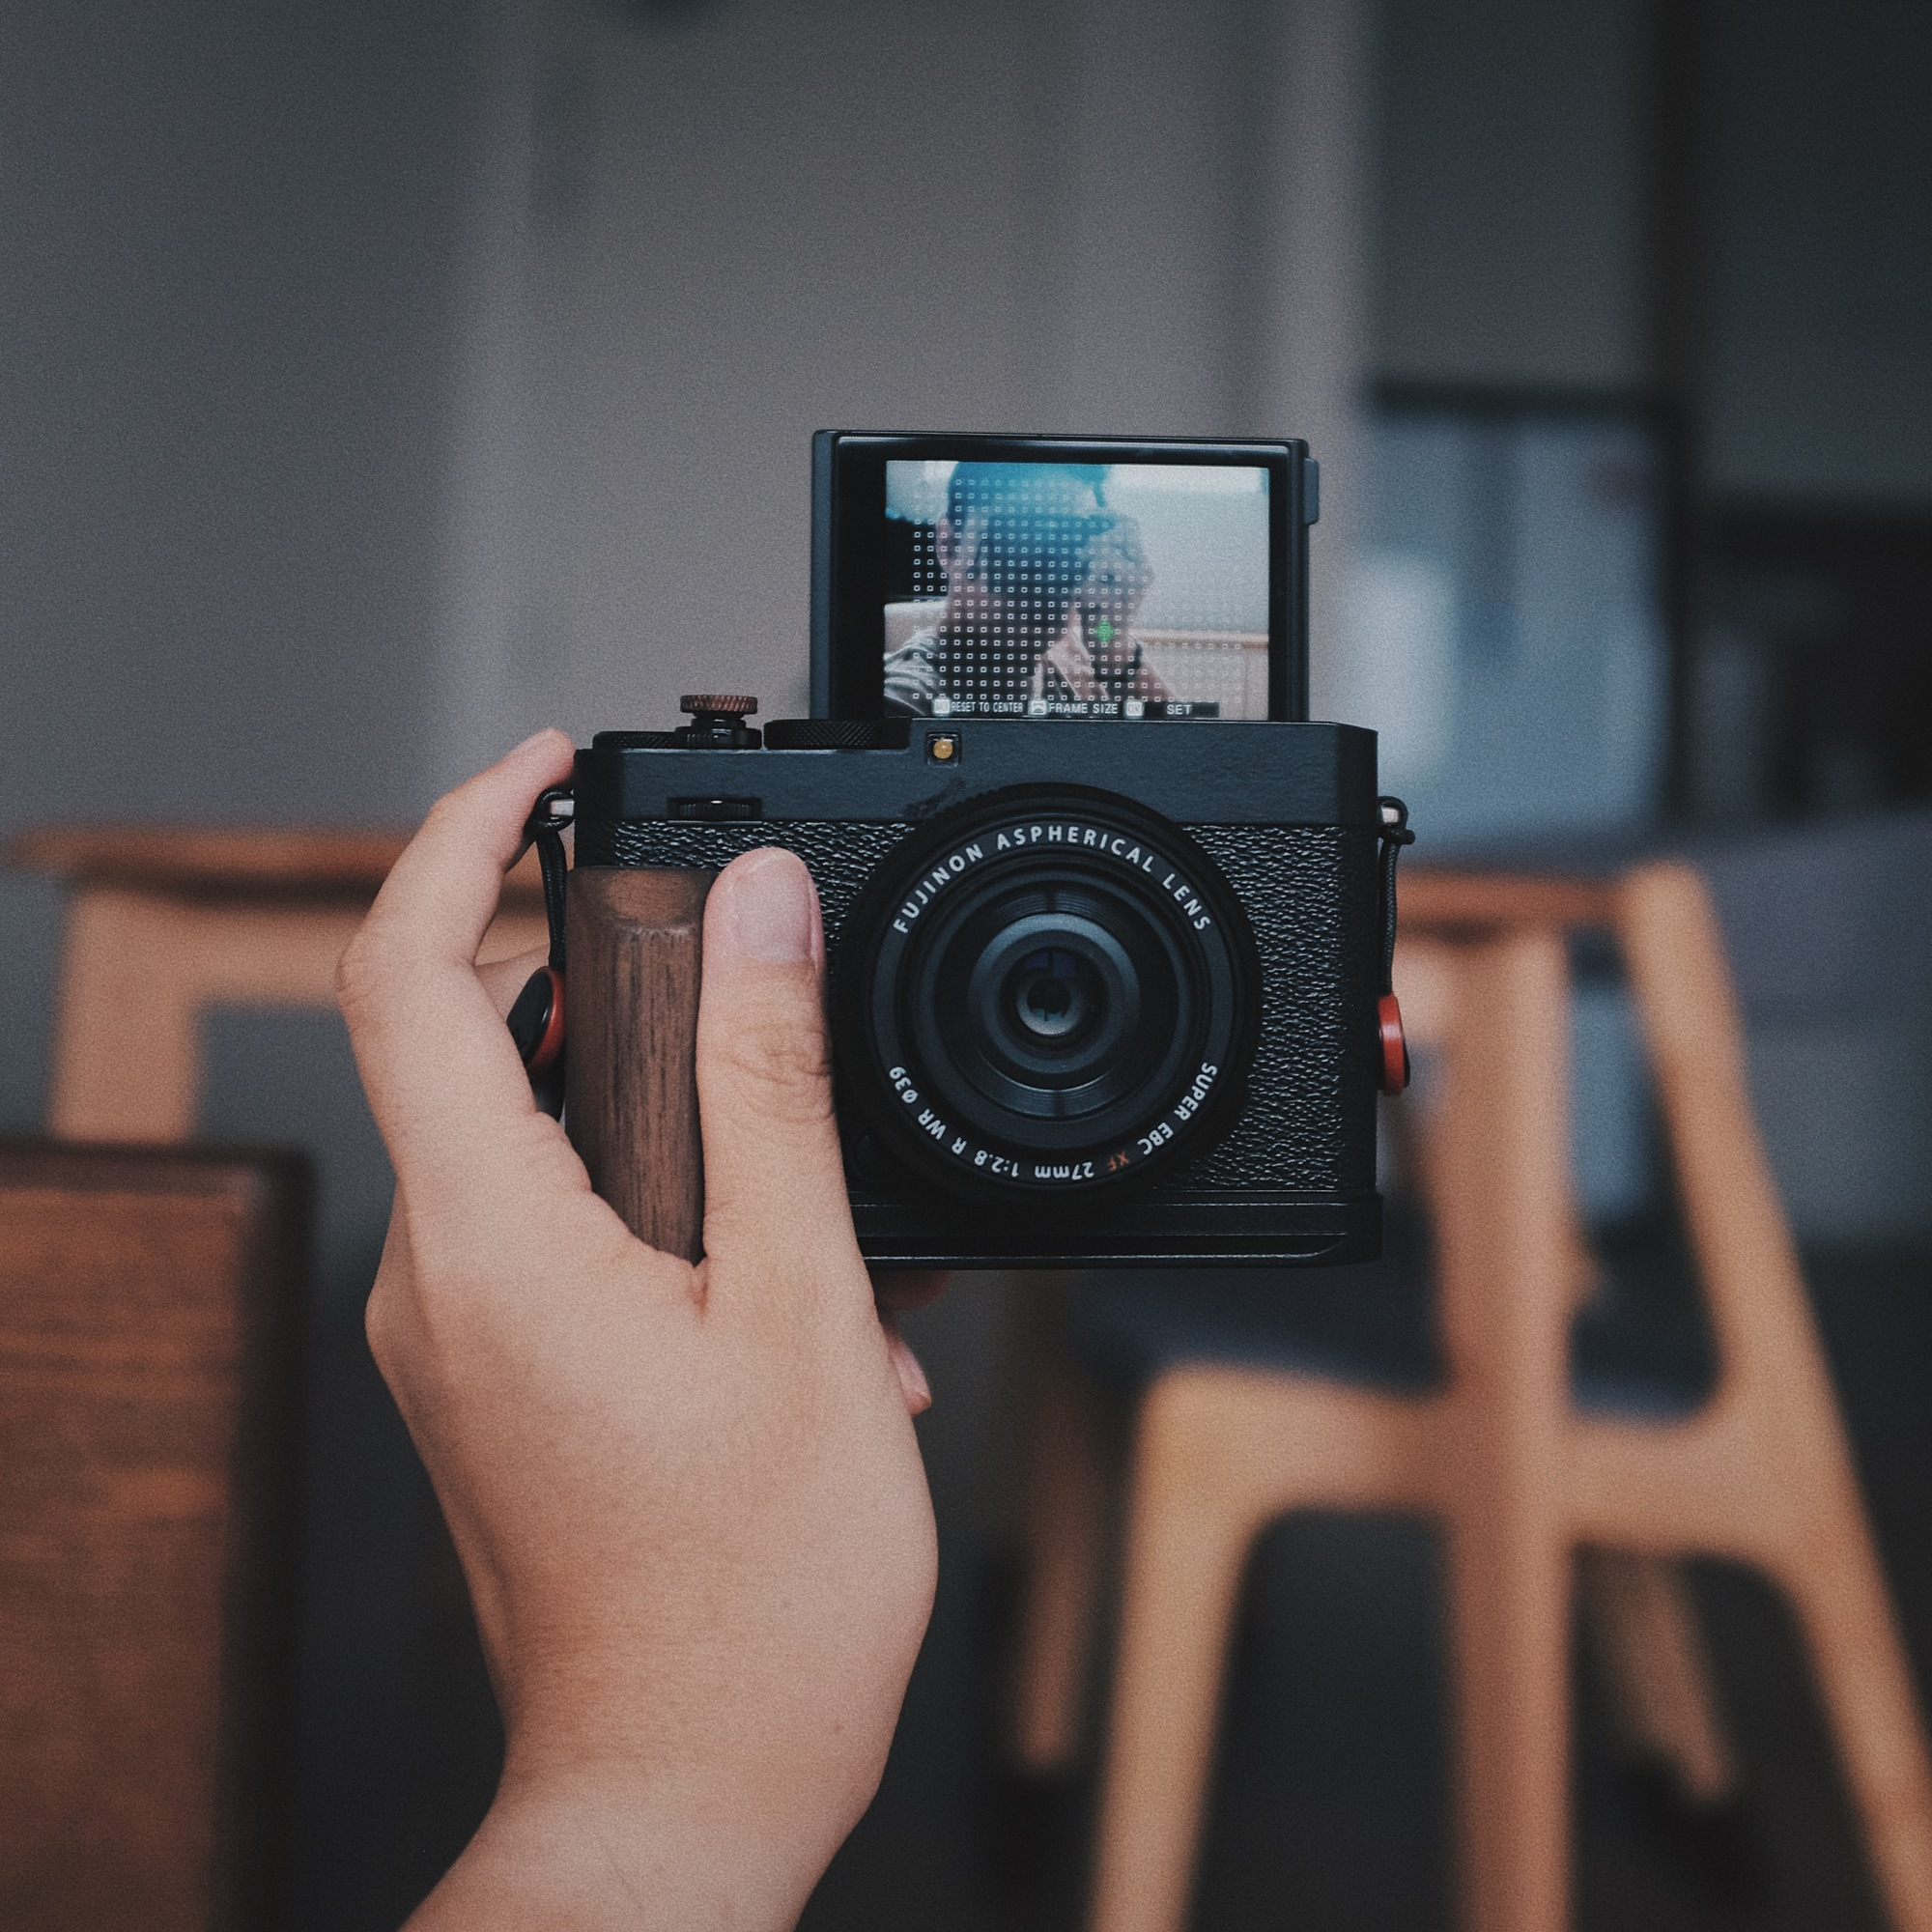
\includegraphics[width=\linewidth]{\envfinaldir/coverpic-prod.jpg}\par
            % \vskip 30pt
            \vfill

            \normalsize\rmfamily\scshape
            \copyright{} The Web Digest Project \hfill\large \envdatestr
        \end{center}
    \end{titlepage}
    % \restoregeometry
}
\newcommand{\simplehref}[1]{%
    \textcolor{blue!80!green}{\href{#1}{#1}}%
}
\renewcommand{\contentsname}{\center\Huge\sffamily\bfseries Contents\par\vskip 20pt}
\newcounter{ipartcounter}
\setcounter{ipartcounter}{0}
\newcommand{\ipart}[1]{
    % \vskip 20pt
    \clearpage
    \stepcounter{ipartcounter}
    \phantomsection
    \addcontentsline{toc}{chapter}{#1}
    % \begin{center}
    %     \Huge
    %     \sffamily\bfseries
    %     #1
    % \end{center}
    % \vskip 20pt plus 7pt
}
\newcounter{ichaptercounter}
\setcounter{ichaptercounter}{0}
\newcommand{\ichapter}[1]{
    % \vskip 20pt
    \clearpage
    \stepcounter{ichaptercounter}
    \phantomsection
    \addcontentsline{toc}{section}{\numberline{\arabic{ichaptercounter}}#1}
    \begin{center}
        \Huge
        \sffamily\bfseries
        #1
    \end{center}
    \vskip 20pt plus 7pt
}
\newcommand{\entrytitlefont}[1]{\subsection*{\raggedright\Large\sffamily\bfseries#1}}
\newcommand{\entryitemGeneric}[2]{
    % argv: title, url
    \parbox{\linewidth}{
        \entrytitlefont{#1}\par\vskip 5pt
        \footnotesize\ttfamily\mdseries
        \simplehref{#2}
    }\vskip 11pt plus 11pt minus 1pt
}
\newcommand{\entryitemGithub}[3]{
    % argv: title, url, desc
    \parbox{\linewidth}{
        \entrytitlefont{#1}\par\vskip 5pt
        \footnotesize\ttfamily\mdseries
        \simplehref{#2}\par\vskip 5pt
        \small\rmfamily\mdseries#3
    }\vskip 11pt plus 11pt minus 1pt
}
\newcommand{\entryitemAp}[3]{
    % argv: title, url, desc
    \parbox{\linewidth}{
        \entrytitlefont{#1}\par\vskip 5pt
        \footnotesize\ttfamily\mdseries
        \simplehref{#2}\par\vskip 5pt
        \small\rmfamily\mdseries#3
    }\vskip 11pt plus 11pt minus 1pt
}
\newcommand{\entryitemHackernews}[3]{
    % argv: title, hnurl, rawurl
    % \parbox{\linewidth}{
    %     \entrytitlefont{#1}\par\vskip 5pt
    %     \footnotesize\ttfamily\mdseries
    %     \simplehref{#3}\par
    %     \textcolor{black!50}{\href{#2}{#2}}
    % }\vskip 11pt plus 11pt minus 1pt
    \begin{minipage}{\linewidth}
            \entrytitlefont{#1}\par\vskip 5pt
            \footnotesize\ttfamily\mdseries
            \simplehref{#3}\par
            \textcolor{black!50}{\href{#2}{#2}}
    \end{minipage}\par\vskip 11pt plus 11pt minus 1pt
}







\begin{document}

\makeheader

\tableofcontents\clearpage




\ipart{Developers}
\ichapter{Hacker News}
\entryitemTwoLinks{Convert photos to Atkinson dithering}{https://news.ycombinator.com/item?id=44212446}{https://gazs.github.io/canvas-atkinson-dither/}

\entryitemTwoLinks{Self-Host and Tech Independence: The Joy of Building Your Own}{https://news.ycombinator.com/item?id=44211273}{https://www.ssp.sh/blog/self-host-self-independence/}

\entryitemTwoLinks{My experiment living in a tent in Hong Kong's jungle}{https://news.ycombinator.com/item?id=44210736}{https://corentin.trebaol.com/Blog/8.+The+Homelessness+Experiment}

\entryitemTwoLinks{Washington Post's Privacy Tip: Stop Using Chrome, Delete Meta Apps (and Yandex)}{https://news.ycombinator.com/item?id=44210689}{https://tech.slashdot.org/story/25/06/07/035249/washington-posts-privacy-tip-stop-using-chrome-delete-metas-apps-and-yandex}

\entryitemTwoLinks{Bill Atkinson has died}{https://news.ycombinator.com/item?id=44210606}{https://daringfireball.net/linked/2025/06/07/bill-atkinson-rip}

\entryitemTwoLinks{After Pornhub left France, this VPN saw a 1,000\% surge in signups in 30 minutes}{https://news.ycombinator.com/item?id=44210557}{https://mashable.com/article/proton-vpn-pornhub-france}

\entryitemTwoLinks{Hate Radio (2011)}{https://news.ycombinator.com/item?id=44209833}{https://rwandanstories.org/genocide/hate\_radio.html}

\entryitemTwoLinks{Musk-Trump dispute includes threats to SpaceX contracts}{https://news.ycombinator.com/item?id=44209515}{https://spacenews.com/musk-trump-dispute-includes-threats-to-spacex-contracts/}

\entryitemTwoLinks{What was Radiant AI, anyway?}{https://news.ycombinator.com/item?id=44209497}{https://blog.paavo.me/radiant-ai/}

\entryitemTwoLinks{Why We're Moving on from Nix}{https://news.ycombinator.com/item?id=44208968}{https://blog.railway.com/p/introducing-railpack}

\entryitemTwoLinks{A tool for burning visible pictures on a compact disc surface}{https://news.ycombinator.com/item?id=44208283}{https://github.com/arduinocelentano/cdimage}

\entryitemTwoLinks{Low-Level Optimization with Zig}{https://news.ycombinator.com/item?id=44208060}{https://alloc.dev/2025/06/07/zig\_optimization}

\entryitemTwoLinks{Windows 10 spies on your use of System Settings (2021)}{https://news.ycombinator.com/item?id=44208050}{https://www.michaelhorowitz.com/Windows10.spying.onsettings.php}

\entryitemTwoLinks{The FAIR Package Manager: Decentralized WordPress infrastructure}{https://news.ycombinator.com/item?id=44207503}{https://joost.blog/path-forward-for-wordpress/}

\entryitemTwoLinks{Getting Past Procrastination}{https://news.ycombinator.com/item?id=44207095}{https://spectrum.ieee.org/getting-past-procastination}

\entryitemTwoLinks{Reverse Engineering Cursor's LLM Client}{https://news.ycombinator.com/item?id=44207063}{https://www.tensorzero.com/blog/reverse-engineering-cursors-llm-client/}

\entryitemTwoLinks{Why are smokestacks so tall?}{https://news.ycombinator.com/item?id=44206553}{https://practical.engineering/blog/2025/6/3/why-are-smokestacks-so-tall}

\entryitemTwoLinks{I read all of Cloudflare's Claude-generated commits}{https://news.ycombinator.com/item?id=44205697}{https://www.maxemitchell.com/writings/i-read-all-of-cloudflares-claude-generated-commits/}

\entryitemTwoLinks{Medieval Africans had a unique process for purifying gold with glass (2019)}{https://news.ycombinator.com/item?id=44205599}{https://www.atlasobscura.com/articles/medieval-african-gold}

\entryitemTwoLinks{Falsehoods programmers believe about aviation}{https://news.ycombinator.com/item?id=44205590}{https://flightaware.engineering/falsehoods-programmers-believe-about-aviation/}\ichapter{GitHub}
\entryitemWithDescription{\hskip 0pt{}vinta/awesome-python}{https://github.com/vinta/awesome-python}{An opinionated list of awesome Python frameworks, libraries, software
and resources.\\
Language: Python\\
Stars: 245875\\
Forks: 25762}\ichapter{Dribbble}
\entryitemGeneric{\hskip 0pt{}Aquasan}{https://dribbble.com/shots/26100535-Aquasan}

\entryitemGeneric{\hskip 0pt{}Eagle}{https://dribbble.com/shots/26099428-Eagle}

\entryitemGeneric{\hskip 0pt{}Mnp Technologies - Logo Design}{https://dribbble.com/shots/26092034-Mnp-Technologies-Logo-Design}

\entryitemGeneric{\hskip 0pt{}Singular Logo Concept (Unused)}{https://dribbble.com/shots/26091755-Singular-Logo-Concept-Unused}

\entryitemGeneric{\hskip 0pt{}Cre8tera // Website}{https://dribbble.com/shots/26091009-Cre8tera-Website}

\entryitemGeneric{\hskip 0pt{}Cool Pool Logo Design - Letter C Monogram}{https://dribbble.com/shots/26091401-Cool-Pool-Logo-Design-Letter-C-Monogram}

\entryitemGeneric{\hskip 0pt{}Gorilla + Bar Chart Logo}{https://dribbble.com/shots/26092670-Gorilla-Bar-Chart-Logo}

\entryitemGeneric{\hskip 0pt{}zeero logo design}{https://dribbble.com/shots/26087342-zeero-logo-design}

\entryitemGeneric{\hskip 0pt{}Create email inbox composition}{https://dribbble.com/shots/26083118-Create-email-inbox-composition}

\entryitemGeneric{\hskip 0pt{}Shori Brand}{https://dribbble.com/shots/26088139-Shori-Brand}

\entryitemGeneric{\hskip 0pt{}Roaring Bear}{https://dribbble.com/shots/26087788-Roaring-Bear}

\entryitemGeneric{\hskip 0pt{}Eagle}{https://dribbble.com/shots/26085536-Eagle}

\entryitemGeneric{\hskip 0pt{}Hand-drawn illustration pack}{https://dribbble.com/shots/26084735-Hand-drawn-illustration-pack}

\entryitemGeneric{\hskip 0pt{}Dog Mascot Various Poses}{https://dribbble.com/shots/26087977-Dog-Mascot-Various-Poses}

\entryitemGeneric{\hskip 0pt{}Branding Concept for Europe}{https://dribbble.com/shots/26087652-Branding-Concept-for-Europe}

\entryitemGeneric{\hskip 0pt{}B2B Dashboard \& Web App UI UX Design for Carbon Solutions}{https://dribbble.com/shots/26076624-B2B-Dashboard-Web-App-UI-UX-Design-for-Carbon-Solutions}

\entryitemGeneric{\hskip 0pt{}Patriot Logo Design (Unused for Sale)}{https://dribbble.com/shots/26081047-Patriot-Logo-Design-Unused-for-Sale}

\entryitemGeneric{\hskip 0pt{}Heliopoint}{https://dribbble.com/shots/26081987-Heliopoint}

\entryitemGeneric{\hskip 0pt{}Apple}{https://dribbble.com/shots/26084067-Apple}

\entryitemGeneric{\hskip 0pt{}Illustration}{https://dribbble.com/shots/26083223-Illustration}

\entryitemGeneric{\hskip 0pt{}Europe Logo Animation}{https://dribbble.com/shots/26082596-Europe-Logo-Animation}

\entryitemGeneric{\hskip 0pt{}Arc Logo}{https://dribbble.com/shots/26083648-Arc-Logo}

\entryitemGeneric{\hskip 0pt{}Heyo Turns 2!}{https://dribbble.com/shots/26078572-Heyo-Turns-2}

\entryitemGeneric{\hskip 0pt{}Fox Brand Mascot}{https://dribbble.com/shots/26077954-Fox-Brand-Mascot}


\ipart{Developers~~~~(zh-Hans)}
\ichapter{Solidot}
\entryitemGeneric{\hskip 0pt{}天文学家发现中等质量黑洞的新证据}{https://www.solidot.org/story?sid=81495}

\entryitemGeneric{\hskip 0pt{}英国考虑推出数字 ID 卡}{https://www.solidot.org/story?sid=81494}

\entryitemGeneric{\hskip 0pt{}就读美国大学的中国留学生人数持续下降}{https://www.solidot.org/story?sid=81493}

\entryitemGeneric{\hskip 0pt{}YouTube 以有害内容下架主播的自我托管视频内容的教程}{https://www.solidot.org/story?sid=81492}

\entryitemGeneric{\hskip 0pt{}德国数字部长呼吁在开放标准和开源的原则下开发欧洲 IT 解决方案}{https://www.solidot.org/story?sid=81490}

\entryitemGeneric{\hskip 0pt{}阿里云遭遇域名解析故障}{https://www.solidot.org/story?sid=81489}

\entryitemGeneric{\hskip 0pt{}科学家通过脑机接口恢复失明动物视觉功能}{https://www.solidot.org/story?sid=81488}

\entryitemGeneric{\hskip 0pt{}日 ispace 登月尝试再次失败}{https://www.solidot.org/story?sid=81487}

\entryitemGeneric{\hskip 0pt{}加州法庭裁决驾驶时在手机上查地图违法}{https://www.solidot.org/story?sid=81486}

\entryitemGeneric{\hskip 0pt{}海南政府试点跨境加速服务}{https://www.solidot.org/story?sid=81485}

\entryitemGeneric{\hskip 0pt{}在传出 OpenAI 准备收购 Windsurf 后 Anthropic 切断了该公司对其大模型的访问}{https://www.solidot.org/story?sid=81484}

\entryitemGeneric{\hskip 0pt{}亚马逊测试用人形机器人送包裹}{https://www.solidot.org/story?sid=81483}

\entryitemGeneric{\hskip 0pt{}美洲原住民在千年前就以集约化方式种植玉米}{https://www.solidot.org/story?sid=81482}

\entryitemGeneric{\hskip 0pt{}Adobe 发布 Android 版 Photoshop,目前免费测试}{https://www.solidot.org/story?sid=81481}

\entryitemGeneric{\hskip 0pt{}特斯拉汽车销量在欧洲继续下滑}{https://www.solidot.org/story?sid=81480}

\entryitemGeneric{\hskip 0pt{}Wendelstein 7-X 仿星器创下可控核聚变新纪录}{https://www.solidot.org/story?sid=81479}

\entryitemGeneric{\hskip 0pt{}Google Chrome 撤销对中华电信和 Netlock CA 的信任}{https://www.solidot.org/story?sid=81478}

\entryitemGeneric{\hskip 0pt{}随着 Windows 10 即将终止支持,KDE 项目试图吸引微软用户}{https://www.solidot.org/story?sid=81477}

\entryitemGeneric{\hskip 0pt{}草帽星系可能经历过星系合并}{https://www.solidot.org/story?sid=81476}

\entryitemGeneric{\hskip 0pt{}科学家发现一颗位于宜居带的超级地球}{https://www.solidot.org/story?sid=81475}\ichapter{V2EX}
\entryitemGeneric{\hskip 0pt{}[宽带症候群] 关于青海的家庭宽带出口 IP 频繁变化}{https://www.v2ex.com/t/1137121}

\entryitemGeneric{\hskip 0pt{}[问与答] yb 上最喜欢的两位博主,他们的交流看起来真的很轻松愉快}{https://www.v2ex.com/t/1137120}

\entryitemGeneric{\hskip 0pt{}[问与答] 在线/离线本例 html 转为 markdown 有什么好用工具吗?}{https://www.v2ex.com/t/1137119}

\entryitemGeneric{\hskip 0pt{}[问与答] Window10 无法连接 WPA3 的无线 AP , 怎么解决?}{https://www.v2ex.com/t/1137118}

\entryitemGeneric{\hskip 0pt{}[问与答] 2025 年了 闲置手机 改装 为小型服务器 有什么比较完善优秀的方案吗?}{https://www.v2ex.com/t/1137117}

\entryitemGeneric{\hskip 0pt{}[程序员] 网站开发小白设想了一个存储在 s3 上的静态照片/视频网站,仅供家人访问,请问是否可行?}{https://www.v2ex.com/t/1137115}

\entryitemGeneric{\hskip 0pt{}[分享发现] 微软账号被盗了,大家最好注意一下。}{https://www.v2ex.com/t/1137114}

\entryitemGeneric{\hskip 0pt{}[macOS] 系统语言切换为英文后,右键菜单里很多项目仍显示中文?一次关于 LaunchServices 本地化注册机制的深挖过程}{https://www.v2ex.com/t/1137113}

\entryitemGeneric{\hskip 0pt{}[问与答] 车祸事故后,对方出院两个月后挂了,对方想要更多的赔偿,我们怎么应对?}{https://www.v2ex.com/t/1137111}

\entryitemGeneric{\hskip 0pt{}[分享发现] Cybernews: 可能是有史以来侵袭中国最严重的数据泄露事件}{https://www.v2ex.com/t/1137110}

\entryitemGeneric{\hskip 0pt{}[硬件] 对于小键盘真的没什么用吗?}{https://www.v2ex.com/t/1137109}

\entryitemGeneric{\hskip 0pt{}[宽带症候群] 移动、电信互联这么慢,有什么办法?}{https://www.v2ex.com/t/1137108}

\entryitemGeneric{\hskip 0pt{}[Linux] aws 的 ubuntu 机器, 怎么才能实现直接 root 密码登录}{https://www.v2ex.com/t/1137107}

\entryitemGeneric{\hskip 0pt{}[问与答] 关于车辆事故的问题}{https://www.v2ex.com/t/1137106}

\entryitemGeneric{\hskip 0pt{}[生活] 爷爷病重在医院,跟踪照顾的一天写下了这段话,求困境建议}{https://www.v2ex.com/t/1137105}

\entryitemGeneric{\hskip 0pt{}[站长] 最近打算优化一下自己中二的网站,大佬们给点建议}{https://www.v2ex.com/t/1137104}

\entryitemGeneric{\hskip 0pt{}[投资] 昨天美股又亏了 20 万,怎么办?}{https://www.v2ex.com/t/1137102}

\entryitemGeneric{\hskip 0pt{}[Apple] 升级到了 MacOS Sequoia 15.5 系统级支持 markdown 预览}{https://www.v2ex.com/t/1137101}

\entryitemGeneric{\hskip 0pt{}[问与答] svg 图标在网页上锯齿状明显}{https://www.v2ex.com/t/1137096}

\entryitemGeneric{\hskip 0pt{}[问与答] 最近网络总是有问题,访问一些网站或者 app 会卡顿}{https://www.v2ex.com/t/1137094}

\entryitemGeneric{\hskip 0pt{}[iPad] iPad 扩展坞频繁断连如何解决}{https://www.v2ex.com/t/1137093}

\entryitemGeneric{\hskip 0pt{}[程序员] 适用原生 JS 的场景}{https://www.v2ex.com/t/1137092}

\entryitemGeneric{\hskip 0pt{}[推广] 目前无需存量即可开的券商}{https://www.v2ex.com/t/1137091}

\entryitemGeneric{\hskip 0pt{}[NAS] 威联通如何在保留 emmc 的情况下安装 pve}{https://www.v2ex.com/t/1137090}

\entryitemGeneric{\hskip 0pt{}[Minecraft] Java 原版服务器招新 基岩可进}{https://www.v2ex.com/t/1137089}

\entryitemGeneric{\hskip 0pt{}[Windows] win11 如何删除程序卸载后遗留的右键菜单}{https://www.v2ex.com/t/1137088}

\entryitemGeneric{\hskip 0pt{}[分享创造] 图片背景 AI 去除工具,用来扣图片背景图灰常不错!}{https://www.v2ex.com/t/1137087}

\entryitemGeneric{\hskip 0pt{}[问与答] 如果要办一张国内的万事达或者 VISA 信用卡,推荐办哪个}{https://www.v2ex.com/t/1137084}

\entryitemGeneric{\hskip 0pt{}[分享创造] 红枫笔记: 一个有些不一样的 Usememos/Blinko/AI 客户端}{https://www.v2ex.com/t/1137083}

\entryitemGeneric{\hskip 0pt{}[推广] 个人开源项目 MCPHub,一站式管理和聚合 MCP 服务器}{https://www.v2ex.com/t/1137082}

\entryitemGeneric{\hskip 0pt{}[VPS] 东南亚的 VPS 有哪些?}{https://www.v2ex.com/t/1137081}

\entryitemGeneric{\hskip 0pt{}[Apple] Apple Watch Series5 用户,想要知道秋季 11 代有没有换的必要}{https://www.v2ex.com/t/1137079}

\entryitemGeneric{\hskip 0pt{}[问与答] 一觉醒来,手环挂壁了}{https://www.v2ex.com/t/1137078}

\entryitemGeneric{\hskip 0pt{}[游戏] 游戏变速器 OpenSpeedy v1.7.0 发布}{https://www.v2ex.com/t/1137077}

\entryitemGeneric{\hskip 0pt{}[问与答] 求助一个 SSL 证书问题}{https://www.v2ex.com/t/1137076}

\entryitemGeneric{\hskip 0pt{}[酷工作] 我因为在美团面活水被光速开除}{https://www.v2ex.com/t/1137075}

\entryitemGeneric{\hskip 0pt{}[生活] 你好啊,美好的周六晚上!}{https://www.v2ex.com/t/1137074}

\entryitemGeneric{\hskip 0pt{}[问与答] 有什么优惠的购买拯救者 Y9000P/X 的渠道吗?}{https://www.v2ex.com/t/1137073}

\entryitemGeneric{\hskip 0pt{}[问与答] WSL 转换稀疏矩阵失败}{https://www.v2ex.com/t/1137070}

\entryitemGeneric{\hskip 0pt{}[macOS] 哪个软件可以显示 WiFi 速率}{https://www.v2ex.com/t/1137069}

\entryitemGeneric{\hskip 0pt{}[分享创造] 查询本机访问不同网站的公网 IP 的网站。可用于检测代理分流,避免被 AI 工具封号}{https://www.v2ex.com/t/1137068}

\entryitemGeneric{\hskip 0pt{}[分享创造] 🎉 新版本的 海棠诗社 上线啦!}{https://www.v2ex.com/t/1137067}

\entryitemGeneric{\hskip 0pt{}[分享发现] 告诉大家一个百万播放的流量密码,最近在海外平台真的太火爆了}{https://www.v2ex.com/t/1137066}

\entryitemGeneric{\hskip 0pt{}[问与答] 你们真能遇到傻 x 一笑而过吗}{https://www.v2ex.com/t/1137065}

\entryitemGeneric{\hskip 0pt{}[问与答] 有没有类似趣发电这种可以不用登录就购买虚拟商品的平台}{https://www.v2ex.com/t/1137064}

\entryitemGeneric{\hskip 0pt{}[音乐] 现在听歌你们是用 Apple Music / Spotify 还是 网易云 / Q 音?}{https://www.v2ex.com/t/1137063}

\entryitemGeneric{\hskip 0pt{}[职场话题] 请教北美大佬,想从数仓 DE 转成做数据流的 DE, AWS Certified DE 证书在面试的时候有一点加成吗?}{https://www.v2ex.com/t/1137062}

\entryitemGeneric{\hskip 0pt{}[OpenWrt] 刷机还是京东云的雅典娜方便}{https://www.v2ex.com/t/1137061}

\entryitemGeneric{\hskip 0pt{}[macOS] 求 mac 下的 everything}{https://www.v2ex.com/t/1137060}

\entryitemGeneric{\hskip 0pt{}[VPS] 免费无限流量 VPS 申请}{https://www.v2ex.com/t/1137059}


\ipart{Generic News}
\ichapter{联合早报}
\entryitemWithDescription{美中6月9日伦敦会谈料聚焦稀土科技关税 学者:有望取得实质进展}{https://www.zaobao.com/news/china/story20250607-6605709}{美中领导人通话不到两天,美国总统特朗普星期五(6月6日)率先宣布,美方经贸官员将于星期一(6月9日)在伦敦与中方代表举行会谈。他也称,北京已同意恢复向美国供应稀土。 中国外交部发言人星期六(6月7日)晚随后证实,称中国国务院副总理何立峰将于6月8日至13日访问英国,其间,将与美方举行中美经贸磋商机制首次会议。 受访学者预料,中美在伦敦会谈将聚焦稀土、科技与关税等议题……}

\entryitemWithDescription{领导人峰会在即 中欧就电动车稀土等贸易问题取得进展}{https://www.zaobao.com/news/china/story20250607-6610128}{中欧领导人峰会在即,持续困扰双边关系的诸多贸易问题正取得进展,双方为中国产电动车制定最低价格的谈判进入最后阶段,北京也表态愿放宽对欧稀土出口,并将于7月5日前对欧盟白兰地反倾销案作出最终裁定……}

\entryitemWithDescription{民进党:最多可罢免10席以上国民党立委}{https://www.zaobao.com/news/china/story20250607-6606110}{(台北综合讯)台湾将在7月至8月启动罢免投票,执政的民进党内部评估认为,虽有多名党籍立委被连署提案罢免,但成功罢免的可能性不高;相较之下,国民党则可能有超过10席立委面临被罢免成功的风险。 综合《联合报》《上报》等报道,民进党人士分析,国民党原本认为原住民族选区``蓝大于绿'',因此率先对该选区的民进党立委陈莹与伍丽华发起罢免,未料两案第二阶段连署相继失败,重挫士气……}

\entryitemWithDescription{吉利董事长:汽车工业存在``严重的产能过剩''}{https://www.zaobao.com/news/china/story20250607-6609477}{(北京路透电)吉利控股集团董事长李书福说,当今世界的汽车工业存在``严重的产能过剩'',该公司已决定不再建设新的汽车生产工厂或扩大现有工厂的产能。 李书福星期六(6月7日)以视频方式参加在重庆举行的``中国汽车重庆论坛'',并发表上述讲话。 他说,吉利不搞重复建设,而要充分利用全球过剩的产能,尽最大可能地展开务实合作、资源重组……}

\entryitemWithDescription{台籍教师持中国大陆定居证遭废台湾身份 批陆委会非法滥权}{https://www.zaobao.com/news/china/story20250607-6606366}{(台北综合讯)在福建任教的台籍教师张立齐因持有中国大陆定居证被废止台湾身份,他随后批评台湾政府的大陆委员会``非法滥权迫害'',陆委会则回应称``少数人不要心存侥幸,挑战政府执法决心''。 综合《自由时报》《中国时报》报道,在福建华侨大学任教的张立齐,去年响应中国大陆融合发展政策,成为福建首名领取``台湾居民定居证''的台湾人……}

\entryitemWithDescription{美指控中国研究人员走私危险真菌引质疑 中领馆批政治操弄}{https://www.zaobao.com/news/china/story20250607-6604686}{(芝加哥综合讯)两名中国研究人员在美国被控走私``潜在农业恐袭武器''真菌入境后,农业专家质疑称相关真菌在美已广泛存在且风险极小,中国官方也批评美方借此搞政治操弄。 美国司法部6月3日宣布起诉密歇根大学一名中国籍研究生和她在中国大学进行同类研究的男友,指控他们涉嫌将能引发农作物灾害的禾谷镰刀菌走私到美国……}

\entryitemWithDescription{时隔两个月 波音恢复对华交付商用飞机}{https://www.zaobao.com/news/china/story20250607-6605169}{(西雅图综合讯)美国航空巨头波音自4月以来首次恢复向中国交付商用飞机,显示中美双边贸易在关税僵局的背景下正逐步回暖。 综合路透社和彭博社报道,FlightRadar24的飞行数据显示,一架注册编号为N230BE、涂有厦门航空标志的波音737 MAX客机于星期五(6月6日)早上10时从西雅图起飞,开启飞往中国交付中心的首段航程……}

\entryitemWithDescription{新闻人间:国民党的新``战神''蒋万安}{https://www.zaobao.com/news/china/story20250607-6590758}{向来温文有礼的国民党籍台北市长蒋万安,因不满行政院克扣地方政府的一般性补助款,继上周率先提起诉愿后,星期四(6月5日)又带着九位同党籍的县市长和代表赴行政院请愿,强调``我们拒绝任中央宰割''。 行政院长卓荣泰反驳说,行政院已经没钱缴电费,``我们自己都无力自保,何来宰割……}

\entryitemWithDescription{于泽远:中国再秀``核肌肉''}{https://www.zaobao.com/news/china/story20250607-6584360}{中国官媒央视6月2日公开了东风-5洲际导弹的具体参数,这是去年9月解放军向南太平洋海域发射携载训练模拟弹头的东风-31AG洲际弹道导弹后,中国再次秀出``核肌肉''……}

\entryitemWithDescription{中国和南亚国家贸易额10年间翻番}{https://www.zaobao.com/news/china/story20250606-6588580}{(北京综合讯)中国和南亚国家贸易额10年间翻番,在2024年达近2000亿美元(2570亿新元)。 综合新华社与央视新闻报道,中国商务部副部长鄢东星期五(6月6日)在发布会上介绍,近10年来,中国和南亚国家贸易额年均增长率约6.3\%,中国连续多年成为巴基斯坦、孟加拉国等国最大贸易伙伴。 他说,尼泊尔的羊绒制品、阿富汗的青金石、印度的珠宝、斯里兰卡的茶叶香料等南亚商品,广受中国消费者好评……}

\entryitemWithDescription{中美僵持 美国驻华大使安抚美企}{https://www.zaobao.com/news/china/story20250606-6585694}{(北京综合讯)中美经贸关系僵持不下,给商业界带来巨大的不确定性。美国驻中国大使庞德伟于大使馆接待在华美国商业代表,向美企给予支持和安抚。 庞德伟星期五(6月6日)在X平台发文,表示与美国业界协会美中贸易全国委员会、中国美国商会,及上海美国商会进行了``良好会面'',让他更了解在华美企面临的挑战……}

\entryitemWithDescription{日欧美车企受中国稀土管制波及 分析:军民用途难分所致}{https://www.zaobao.com/news/china/story20250605-6575219}{中国收紧稀土出口管制措施,日欧美多家汽车制造商面临生产线停摆危机。对此,中国官方星期四(6月5日)作出回应,强调稀土具明显军民两用属性,实施出口管制属国际通行做法。 受访专家指出,北京此举并非意图将稀土``武器化'',而是为反制美国关税措施、限制美国军工企业的发展。但由于稀土产品军民用途界限模糊,车企供应链难免会受到波及……}

\entryitemWithDescription{中国大陆悬赏通缉台湾资通电军人 掀两岸新一轮法律战}{https://www.zaobao.com/news/china/story20250605-6574873}{在台湾强化查缉公务人员持领中国大陆身份证件,以及艺人与大陆党政军合作之后,中国大陆星期四(6月5日)再对具有强烈抗中色彩的绿营立委沈伯洋祭出制裁,同时也公布20人的台湾资通电军悬赏名单。受访学者研判,两岸围绕国安情报的法律战将会日益激烈……}

\entryitemWithDescription{北京迎来今年首个高温日 最高气温超过摄氏35度}{https://www.zaobao.com/news/china/story20250605-6575398}{(北京综合讯)北京星期四(6月5日)最高气温超过摄氏35度,出现今年首个高温日,较去年提前四天。 据北京市气象台消息,星期四不到中午,代表``北京温度''的南郊观象台气温就已经达到了30摄氏度,午后突破35度高温线,下午4时23分录得白天最高气温值36.5度。其中,全市高温极值出现在丰台世界公园,为39.9度。 北京市气象台星期三(6月4日)已发布高温橙色预警信号……}

\entryitemWithDescription{香港电影院掀结业潮 全港电影院总数已跌至51家}{https://www.zaobao.com/news/china/story20250605-6575140}{曾被誉为``东方好莱坞''的香港电影行业,近年发展萎缩,今年至今已有五家电影院宣布结业,令全港电影院总数跌至51家。 香港电影院线集团嘉禾星期三(6月4日)于社媒专页公布,位于九龙湾商场MegaBox的电影院租约期满,最后营业日为星期天(6月8日)。为了答谢影迷,影院特别预备了一系列优惠及特别场,包括结业日尾场为``经典盲盒场'',以及提供40港元(6.55新元)票价回馈影迷等等……}

\entryitemWithDescription{中国运车货轮起火后被遗弃太平洋 22名船员获救}{https://www.zaobao.com/news/china/story20250605-6574175}{(阿拉斯加综合讯)一艘运送3000辆汽车、其中约有800辆电动车的货轮,在阿拉斯加海岸外起火后被遗弃在太平洋上,22名船员获救,未有伤情报告。 综合路透社和彭博社报道,这艘货轮``晨光号''(Morning Midas)的船东国际船舶管理公司佐迪亚克海运(Zodiac Maritime),星期三(6月4日)发声明通报上述事故……}

\entryitemWithDescription{四川省政府征求民意 拟倍增婚假和陪产假鼓励生育}{https://www.zaobao.com/news/china/story20250605-6573943}{(成都/香港综合讯)在人口萎缩的压力下,中国四川省政府公开征求民意,对当地生育政策进行优化,包括将婚假从目前的五天倍增至高达25天,以及增加生育假。 中国四川省卫生健康委员会上星期五(5月30日)在官网发布《四川省人口与计划生育条例(修正草案征求意见稿)》,吁请民众于6月30日之前提交有关优化当地生育政策的意见……}

\entryitemWithDescription{陈婧:``苏超''爆火之后}{https://www.zaobao.com/news/china/story20250605-6566785}{过去两周,微信里的江苏朋友不约而同地关注一个从没听过的赛事:苏超。有人晒出观赛照片,有人紧跟最新赛程,还有人发帖为主队获胜喝彩。 5月10日开赛的``苏超'',全称是江苏省城市足球联赛,全省13个城市各组一支球队,并以城市命名。据中国媒体报道,每队职业球员不超过三人,其余由学生、教师、快递员等各行各业的足球爱好者组成。 尽管这个业余联赛的球员水准不及职业比赛,但球迷们观赛热情空前高涨……}

\entryitemWithDescription{王毅见美国大使表达不满 中国学者:示意元首通话条件}{https://www.zaobao.com/news/china/story20250604-6564329}{中美近期就履行日内瓦关税协议相互指责。中国外交部长王毅星期二(6月3日)在北京会见新任美国驻华大使庞德伟时,强调中方认真严格落实双方共识,并敦促美方为中美关系``重返正轨创造必要条件''。 美国总统特朗普上周五在社交媒体发文,指责中国``彻底违反''关税协议。白宫官员随后也批评,中国在解除稀土出口限制方面动作迟缓……}

\entryitemWithDescription{为中新重庆项目10周年拉开帷幕 杨莉明本周访渝两天}{https://www.zaobao.com/news/china/story20250604-6566455}{我国数码发展及新闻部长杨莉明,时隔近一年再次访问重庆,为纪念中新(重庆)战略性互联互通示范项目实施10周年拉开帷幕,启动一系列双边互访、会议等活动。 杨莉明表示,中新重庆项目持续发挥重要平台作用,将新加坡和重庆打造成双枢纽,推动东南亚与中国西部地区更深层次、更广泛的区域间互联互通……}






\clearpage
\leavevmode\vfill
\footnotesize

Copyright \copyright{} 2023-2025 Neruthes and other contributors.

This document is published with CC BY-NC-ND 4.0 license.

The entries listed in this newsletter may be copyrighted by their respective creators.

This newsletter is generated by the Web Digest project.

The newsletters are also delivered via Telegram channel \CJKunderline{\href{https://t.me/webdigestchannel}{https://t.me/webdigestchannel}}.\\
RSS feed is available at \CJKunderline{\href{https://webdigest.pages.dev/rss.xml}{https://webdigest.pages.dev/rss.xml}}.

This newsletter is available in PDF at
\CJKunderline{\href{https://webdigest.pages.dev/}{https://webdigest.pages.dev/}}.

The source code being used to generate this newsletter is available at\\
\CJKunderline{\href{https://github.com/neruthes/webdigest}{https://github.com/neruthes/webdigest}}.

This newsletter is also available in
\CJKunderline{\href{http://webdigest.pages.dev/readhtml/\envyear/WebDigest-20250608.html}{HTML}} and
\CJKunderline{\href{https://github.com/neruthes/webdigest/blob/master/markdown/\envyear/WebDigest-20250608.md}{Markdown}}.


\coverpic{https://unsplash.com/photos/beautiful-cherry-blossoms-bloom-against-a-sky-omxwwtNse3k}{Buddy AN}


\end{document}
